%%%%%%%%%%%%%%%%%%% 
% Reminder: Bad At...
%%%%%%%%%%%%%%%%%%% 
\def\title{Two Big Problems}
\begin{frame}{\title}

\begin{center}
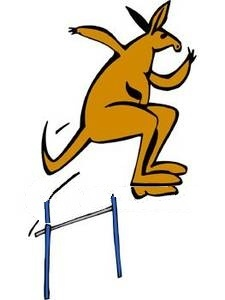
\includegraphics[height=3cm]{../img/hurdle.jpg}
\end{center}

\hh{1. People don't speak in atomic utterances}
\vspace{2ex}

\hh{2. Missing recall: the internet is incomplete} \\
\end{frame}



%%%%%%%%%%%%%%%%%%% 
% Failed Search
%%%%%%%%%%%%%%%%%%% 
\input exampleSearchHeuristic.tex



%%%%%%%%%%%%%%%%%%% 
% Alignment
%%%%%%%%%%%%%%%%%%% 

\tikzset{
  arm angleA/.initial={0},
  arm angleB/.initial={0},
  arm lengthA/.initial={0mm},
  arm lengthB/.initial={0mm},
  arm length/.style={%
    arm lengthA=#1,
    arm lengthB=#1,
  },
  arm/.style={
    to path={%
      (\tikztostart) -- ++(\pgfkeysvalueof{/tikz/arm angleA}:\pgfkeysvalueof{/tikz/arm lengthA}) -- ($(\tikztotarget)+(\pgfkeysvalueof{/tikz/arm angleB}:\pgfkeysvalueof{/tikz/arm lengthB})$) -- (\tikztotarget)
    }
  },
}

%
% The slide
%
\def\title{Lexical Alignment Classifier}
\begin{frame}[fragile]{\title}
\newcommand{\hnode}[1]{|(#1)| \w{#1}}
\newcommand{\rnode}[2]{|(#1#2)| \w{\textcolor<2->{darkblue}{\textbf<2->{#1}}}\only<2->{\textcolor{white}{#2}}}
\newcommand{\bnode}[2]{|(#1#2)| \w{\textcolor<2->{darkblue}{\textcolor<6->{darkred}{\textbf<2->{#1}}}}\only<2->{\textcolor{white}{#2}}}

\begin{tikzpicture}
\matrix[column sep=-0.0em,row sep=1cm,matrix of nodes,row 2/.style={coordinate}] (m) {
% First sentence
\rnode{Forms}{$^p$} & \hnode{of} & \rnode{precipitation}{$^p$} & \bnode{include}{$^p$} & \rnode{rain}{$^p$} & \hnode{and} & \rnode{sleet}{$^p$} \\
\\
% Second sentence
\rnode{Rain}{$^c$} & \hnode{and} & \rnode{snow}{$^c$} & \hnode{are} & \rnode{forms}{$^c$} & \hnode{of} & \rnode{precipitation}{$^c$} \\
};
\only<3->{
\begin{scope}[every path/.style={line width=4pt,white,double=black},every to/.style={arm}, arm angleA=-90, arm angleB=90, arm length=5mm]
 \draw<3-3> (rain$^p$) to (Rain$^c$);
 \draw<3-3> (Forms$^p$) to (forms$^c$);
 \draw<3-3> (precipitation$^p$) to (precipitation$^c$);
 \draw<3-4> (sleet$^p$) to (snow$^c$);
 
 \draw<4-> [draw=green] (rain$^p$) to (Rain$^c$);
 \draw<4-> [draw=green] (Forms$^p$) to (forms$^c$);
 \draw<4-> [draw=green] (precipitation$^p$) to (precipitation$^c$);
 \draw<5-> [draw=red  ] (sleet$^p$) to (snow$^c$);
\end{scope}
}
\end{tikzpicture}

\pause
\pause
\pause
\vspace{2ex}

\hh{Features}
\begin{enumerate}
  \item Matching words
  \pause
  \item Mismatched words
  \pause
  \item Unmatched words in premise/consequent
\end{enumerate}
\pause
\vspace{1ex}
\hh{Competitive with Stanford RTE system (63\% on RTE3)}

\end{frame}



%%%%%%%%%%%%%%%%%%% 
% Lexical + Logic
%%%%%%%%%%%%%%%%%%% 
\def\title{Old Problem: Logic + Lexical Classifiers}
\begin{frame}{\title}
\begin{center}
\hh{FOL and lexical classifiers don't speak the same language} \\
\uncover<2->{\hh{...but natural logic does!}} \\
\vspace{2ex}
\only<1-1>{
\includegraphics[height=4cm]{../img/spy.png}}
\only<2->{
\includegraphics[height=4cm]{../img/speakwhale.jpg}}
\end{center}
\end{frame}



%%%%%%%%%%%%%%%%%%% 
% Evaluation Function
%%%%%%%%%%%%%%%%%%% 
\def\title{Disecting Our Systems}
\begin{frame}{\title}
\hh{Anatomy of a Classifier}
\begin{itemize}
\item Features $f$ (matching / mismatched / unmatched words)
\item Weights $w$
\item Entailment pair $x$; entailment judgment $y \in \{\textrm{entailed}, \textrm{neutral}\}$
\end{itemize}

\begin{center}
$p(y \mid x) 
  = g\left(- w^{\textrm{T}} f(x)\right)
  = \frac{1}{1 + \exp({- w^{\textrm{T}} f(x)})}$
\end{center}
\pause
\vspace{1ex}

\hh{Anatomy of a Search Step}
\begin{enumerate}
\item Mutate a word, or
\item Delete a word, or
\item Insert a word.
\end{enumerate}
\pause
\vspace{1ex}

\begin{center}
\hh{Additive updates on $f(x)$ directly}
\end{center}
\end{frame}



%%%%%%%%%%%%%%%%%%% 
% Evaluation Function
%%%%%%%%%%%%%%%%%%% 


\newcommand{\hnode}[1]{|(#1)| \w{#1}}
\newcommand{\rnode}[2]{|(#1#2)| \w{\textcolor{darkblue}{\textbf{#1}}}\textcolor{white}{#2}}
\newcommand{\bnode}[2]{|(#1#2)| \w{\textcolor{darkblue}{\textcolor{darkred}{\textbf{#1}}}}\textcolor{white}{#2}}

\def\title{Incremental Updates}

%
% Frame 1
%
\begin{frame}[t,fragile]{\title}
\vspace{-5ex}
\begin{center}

\begin{tikzpicture}
\matrix[column sep=-0.0em,row sep=0.75cm,matrix of nodes,row 2/.style={coordinate}] (m) {
% First sentence
\rnode{Forms}{$^p$} & \hnode{of} & \rnode{precipitation}{$^p$} & \bnode{include}{$^p$} & \rnode{rain}{$^p$} & \hnode{and} & \rnode{sleet}{$^p$} \\
\\
% Second sentence
\rnode{Rain}{$^c$} & \hnode{and} & \rnode{snow}{$^c$} & \hnode{are} & \rnode{types}{$^c$} & \hnode{of} & \rnode{precipitation}{$^c$} \\
};
\begin{scope}[every path/.style={line width=4pt,white,double=black},every to/.style={arm}, arm angleA=-90, arm angleB=90, arm length=5mm]
 \draw [draw=green] (rain$^p$) to (Rain$^c$);
 \draw [draw=red] (Forms$^p$) to (types$^c$);
 \draw [draw=green] (precipitation$^p$) to (precipitation$^c$);
 \draw [draw=red  ] (sleet$^p$) to (snow$^c$);
\end{scope}
\end{tikzpicture}
\vspace{1ex}

\hh{Score $w^{\textrm{T}} f(x)$:} -0.5
\vspace{2ex}

\begin{tabular}{lrr}
\textbf{Feature} & \textbf{$w$} & \textbf{$f(x)$} \\
Matching words       &  2.0  & 2 \\
Mismatched words     & -1.0  & 2 \\
Unmatched premise    & -0.5  & 1 \\
Unmatched consequent & -0.75 & 0 \\
Bias                 & -2.0  & 1 
\end{tabular}
\end{center}
\end{frame}


%
% Frame 2
%
\begin{frame}[noframenumbering]{\title}
\exampleTreeLarge{ROOT \\ $~$}
                 {Rain and snow are types of precipitation}
                 {Rain and snow are \textbf{forms} of precipitation}
                 {Rain and snow are types of \textbf{weather}}
\end{frame}


%
% Frame 3
%
\begin{frame}[t,fragile,noframenumbering]{\title}
\vspace{-5ex}
\begin{center}

\begin{tikzpicture}
\matrix[column sep=-0.0em,row sep=0.75cm,matrix of nodes,row 2/.style={coordinate}] (m) {
% First sentence
\rnode{Forms}{$^p$} & \hnode{of} & \rnode{precipitation}{$^p$} & \bnode{include}{$^p$} & \rnode{rain}{$^p$} & \hnode{and} & \rnode{sleet}{$^p$} \\
\\
% Second sentence
\rnode{Rain}{$^c$} & \hnode{and} & \rnode{snow}{$^c$} & \hnode{are} & \rnode{forms}{$^c$} & \hnode{of} & \rnode{precipitation}{$^c$} \\
};
\begin{scope}[every path/.style={line width=4pt,white,double=black},every to/.style={arm}, arm angleA=-90, arm angleB=90, arm length=5mm]
 \draw [draw=green] (rain$^p$) to (Rain$^c$);
 \draw [draw=green] (Forms$^p$) to (forms$^c$);
 \draw [draw=green] (precipitation$^p$) to (precipitation$^c$);
 \draw [draw=red  ] (sleet$^p$) to (snow$^c$);
\end{scope}
\end{tikzpicture}
\vspace{1ex}

\hh{Score $w^{\textrm{T}} f(x)$:} 
  \only<1>{-0.5 + 2 $-$ -1}
  \only<2->{2.5}
\vspace{2ex}

\begin{tabular}{lrr}
\textbf{Feature} & \textbf{$w$} & \textbf{$f(x)$} \\
Matching words       &  2.0  & \textbf{3} \\
Mismatched words     & -1.0  & \textbf{1} \\
Unmatched premise    & -0.5  & 1 \\
Unmatched consequent & -0.75 & 0 \\
Bias                 & -2.0  & 1 
\end{tabular}
\end{center}
\end{frame}


%
% Frame 4
%
\begin{frame}[t,fragile,noframenumbering]{\title}
\vspace{-5ex}
\begin{center}

\begin{tikzpicture}
\matrix[column sep=-0.0em,row sep=0.75cm,matrix of nodes,row 2/.style={coordinate}] (m) {
% First sentence
\rnode{Forms}{$^p$} & \hnode{of} & \rnode{precipitation}{$^p$} & \bnode{include}{$^p$} & \rnode{rain}{$^p$} & \hnode{} & \rnode{}{} \\
\\
% Second sentence
\rnode{Rain}{$^c$} & \hnode{and} & \bnode{snow}{$^c$} & \hnode{are} & \rnode{forms}{$^c$} & \hnode{of} & \rnode{precipitation}{$^c$} \\
};
\begin{scope}[every path/.style={line width=4pt,white,double=black},every to/.style={arm}, arm angleA=-90, arm angleB=90, arm length=5mm]
 \draw [draw=green] (rain$^p$) to (Rain$^c$);
 \draw [draw=green] (Forms$^p$) to (forms$^c$);
 \draw [draw=green] (precipitation$^p$) to (precipitation$^c$);
\end{scope}
\end{tikzpicture}
\vspace{1ex}

\hh{Score $w^{\textrm{T}} f(x)$:} 
  \only<1>{2.5 $-$ -1 $+$ -0.75}
  \only<2->{2.75}
\vspace{2ex}

\begin{tabular}{lrr}
\textbf{Feature} & \textbf{$w$} & \textbf{$f(x)$} \\
Matching words       &  2.0  & 3 \\
Mismatched words     & -1.0  & \textbf{0} \\
Unmatched premise    & -0.5  & 1 \\
Unmatched consequent & -0.75 & \textbf{1} \\
Bias                 & -2.0  & 1 
\end{tabular}
\end{center}
\end{frame}

%%%%%%%%%%%%%%%%%%% 
% Synthesis
%%%%%%%%%%%%%%%%%%% 
\def\title{Why Is This Important?}
\begin{frame}{\title}
\begin{center}

\includegraphics[height=2cm]{../img/efficient.png}
\end{center}

\hh{Search is \textit{efficient}} 
\begin{itemize}
\item \textbf{Speed:} Around 1M search states visited per second
\item \textbf{Memory:} 32 byte search states (store only hash of fact)
\end{itemize}
\vspace{2ex}
\pause

\hh{Speed:} Don't re-featurize at every timestep.
\vspace{2ex}
\pause

\hh{Memory:} Never store intermediate fact as String.
\end{frame}


%%%%%%%%%%%%%%%%%%% 
% Synthesis
%%%%%%%%%%%%%%%%%%% 
\def\title{The Full System}
\begin{frame}{\title}

\hh{Common Sense Facts}
\begin{itemize}
\item Natural logic inference as search
\item Soft relaxation of ``strict'' inference
\item 4x improvement in recall
\end{itemize}
\vspace{1ex}
\pause

\hh{Long Premises}
\begin{itemize}
\item Split the premise into atomic clauses
\item Shorten each clause w/ natural logic
\item 3 F$_1$ improvement on knowledge base population
\end{itemize}
\vspace{1ex}
\pause

\hh{High Recall}
\begin{itemize}
\item Use lexical classifier as evaluation function
\item Detect likely entailment / contradictions
\end{itemize}
\end{frame}

%%%%%%%%%%%%%%%%%%% 
% Results
%%%%%%%%%%%%%%%%%%% 
\def\title{Solving 4$^{th}$ Grade Science}
\begin{frame}{\title}
\hh{Multiple choice questions from real 4$^{th}$ grade science exams}
\begin{center}
\begin{tabular}{lr}
\hline
\textbf{System}                & \multicolumn{1}{c}{\textbf{Accuracy}}  \\
\hline
\sc{Knowbot}                    & 45 \\
\sc{Knowbot (oracle)}           & 57 \\
\hline
\pause
IR Baseline                     & 49 \\
\hline
\pause
NaturalLI                       & 52 \\
NaturalLI + IR                  & 55 \\
\hline
\pause
More Data + IR                  & 62 \\
More Data + IR + NaturalLI      & \textbf{73} \\
\hline
\end{tabular}
\pause
\vspace{2ex}

\hh{We can pass 4$^{th}$ grade science!}

\end{center}

\end{frame}




